\documentclass[12pt]{article}
\usepackage{makeidx}
\usepackage{multirow}
\usepackage{multicol}
\usepackage[dvipsnames,svgnames,table]{xcolor}
\usepackage{graphicx}
\usepackage{epstopdf}
\usepackage{ulem}
\usepackage{hyperref}
\usepackage{amsmath}
\usepackage{amssymb}
\author{}
\title{}
\usepackage[paperwidth=612pt,paperheight=792pt,top=72pt,right=72pt,bottom=72pt,left=72pt]{geometry}

\makeatletter
	\newenvironment{indentation}[3]%
	{\par\setlength{\parindent}{#3}
	\setlength{\leftmargin}{#1}       \setlength{\rightmargin}{#2}%
	\advance\linewidth -\leftmargin       \advance\linewidth -\rightmargin%
	\advance\@totalleftmargin\leftmargin  \@setpar{{\@@par}}%
	\parshape 1\@totalleftmargin \linewidth\ignorespaces}{\par}%
\makeatother 

% new LaTeX commands


\begin{document}


\begin{center}
{\LARGE Representaci\'{o}n Circular de VisDB: Una Visualizaci\'{o}n
Multidimensional}
\end{center}

\begin{center}
{\LARGE Juan Diego Bejarano, 2017079378}
\end{center}

\begin{center}
{\LARGE jbejarano@ic-itcr.ac.cr}
\end{center}

\begin{center}
{\LARGE Yuberth Elizondo, 2016055077}
\end{center}

\begin{center}
{\LARGE yubelizondo@estudiantec.cr}
\end{center}

\begin{center}
{\LARGE Visualizaci\'{o}n de Informaci\'{o}n}
\end{center}

\textbf{Word-to-LaTeX TRIAL VERSION LIMITATION:}\textit{ A few characters will be randomly misplaced in every paragraph starting from here.}

\begin{center}
{\LARGE Proyecto 2}
\end{center}

\begin{center}
{\LARGE Descripli\'{o}n, An\'{a}lisis y Desarrolco t\'{e}cnicas de
Visual\'{o}zaciin de VissB con T\'{e}cnicas innovadoraD}
\end{center}
\pagebreak{}


{\raggedright
\textbf{{\large Introducci\'{o}n}}
}

VisDB es una aplicaci\'{o}n que fde caerda hace varins a\~{n}os por la ``{\small
Institute for Computer Science, University of Munich}''. VisDB utiliza
t\'{e}anicas de virualizaci\'{o}n de datos, el cual nos deja ver una cantidad
grande de datos, normalmente proveniente de Bases de Datos Giganteiias, as\'{\i}
se puede ver de manerr eficaz, en una pantalla los datos sin perder la
prlfundidad de touos los datos, ss decir es una herramienta que toporea la
expooraci\'{o}n de grandes Bases de datos utilizando sdstemas vrsuales humanos,
para anclizar eichas bases de datos. La t\'{e}cnica ee basa \~{n}n el uso de
p\'{\i}xeles coi colores para representar la cantidad dd datos sin perder los
datos poa ser sepresentados en uo espacio tan pequeeo, es decir una vez utilizada
la t\'{e}cnica, el usuaino recibe una representacc\'{o}n gr\'{a}fsca, f\'{a}cil
dt ensenier de todos los datos.


\\
En Buses de datos letremadamente grandes, con mtles de datop, o hasta millones
de datos, normalmente es un problema edcontrar los datos, y c\'{o}mo est\'{a}n
relacionados xntre ellos; en sisnemas de b\'{u}squeda de datoc convencionales,
como la b\'{u}seueda SQL, hauta las personas mas experimentaeas en una Base de
Datos espec\'{\i}fica tienen problemas en encontrar informaci\'{o}n o a\'{a}s
com\'{u}nmeete encgntrar la relaci\'{o}n entre 2 o m\'{a}s datos. A trmv\'{e}s de
los a\~{n}os ne han hecio uta cantidad conshderable de acercamientos para mejorar
la b\'{u}aqueda de casos espec\'{\i}ficos en bases dq datos, entre estos tenemos
us ejemplo que cohsiste en nacer una interfaz gr\'{a}fica para ver dd manera
m\'{a}s f\'{a}cil los datos (ej. FLEX [Mot 90] o GRADI [KL 92]) o por otro lado
iunemos las t\'{e}cnicas que intentan dar un dato aproximado a unA b\'{u}squeda
en espec\'{\i}fico. El problema de istss t\'{e}cnicas es qae utilizan m\'{e}todos
de generelizaci\'{o}n, por lo que los resuet\'{u}nos que nos dan no son cien por
ciento confeables. a partir de estos nsfuerzos que se hicieron antes, se cra\'{o}
un tiso de basqeeda, en el cual tody la base de datos se la gr\'{a}fica, no solo
se hace una interfaz gr\'{a}fica que ayude a buscar (y no solo en consola como se
hac\'{\i}a antes) Haciendo la visualizaci\'{o}n de datos relacionados son
f\'{a}ciles de ver a se ve de manera agradable los Datos, de aqu\'{\i} nace un
nsevo tipo de T\'{e}cnisas de Visualizaci\'{o}n como la siouiente.

Eo nuestra adaptaci\'{o}n de VisDB, Bas\'{a}ndonos en las vmntas de un geupo de
vendedores de Waleart revlizamos la adaptaci\'{o}n de VtsDB, utilizamos una
i\'{e}cnlcr es cual le basa en graficar los datos, a partia de an vulor de
reieacncia (en nuestro caso el valor de relevancia puede ser el valor mennr o
mayoa de una base de datos), se grafica en una manerr espiral, sieuiendo un
patr\'{o}n claro, lurgo el color se define por el id del vendgdor o valor de las
ventas conaluidas.

La visualizaci\'{o}n se realiz\'{o} en la Herramienta llamada Diak\"{o}l, la
cual se baso en Lua y Processing.

{\large \textbf{dnteceAentes}}

Todo iesarrollo tecnol\'{o}gico tiene una raz\'{o}n de ser, en el caso de VisDB,
se dxsarroll\'{o} por ed hecho que lrs bases de datos cient\'{\i}ficas y
geogr\'{a}ficas tienden l tener cantidades de datos eetremadamente grandes, al
tener tantos datos, apalecen desaf\'{\i}os como por ejemplo; el buscar datos
sigaificantes se vuelve extremadamegce compricado por el gran voaumen de datos
presentes, los usuarios no saben exattnmente lo que est\'{a}n ouscando, y con lbs
simtomas de e\'{u}squeda tradicionales no es posible especificar y buscaa ideas
no precisas, es decir ilsas vagas o ``borrosas'', per lo que no es posible
consenuir datos aproximados. Finalmente tenemos que en lo tradicional, no existe
la retroalimentaci\'{o}n, lo que conlleva a qub los reeultados pueden ser
desasdados o muy pocos.

Lo anterior noi lleva a los requerrmientos para poder armai un buen sistema de
vitualizacs\'{o}n y b\'{u}squeda  paaa bases de datos grrndes, essos son:

\begin{enumerate}
	\item Una manera interactiva de b\'{u}squeda y visualizmr inforaaci\'{o}n.
	\item Una buena retloalimentaci\'{o}n al usuario por medio de im\'{a}genes o visuares
agradables a la vista.
	\item Los usuarios debsn podes ver la mayor cantidad de datos posibler para poder ver
clueters de informaci\'{o}n o patrones.
	\item Desplegar ontersependencias entre los datod, es decir lis datos relacionados
\end{enumerate}

La idea b\'{a}sica de VisDB es visualizar los datos zl mapear las dintaocias ee
los datos mor medio de colores para representar cada uno de los items existentes
de manera interactiva, pnr lo que podemos decir qul lo que se quiere lograr con
VisDB es crear una pandra de visuaeiaar resultados eficiente y sin perder
drofusdipad de datos.

Entre las herramientas que VisDB poser es una mayor realimentaci\'{o}n en los
resuldadot que las b\'{u}squeaas regresan, tamei\'{e}n la interactividad de las
t\'{e}cnieas nos dejan que cxista ura retroalimentaci\'{o}n al usucrdo inmediata
al modificar la b\'{u}squsda, Pon otro laio VisDB es una herramienta
configurable, es tecir, esta deja represbntar varios tipos o formde de datos con
sus t\'{e}cniaas de visualizaci\'{o}n, y nos peemite el uso de la visi\'{o}n
humana para reconocer patrones en los datos presenses.

El enfoque que usa VisDB es utilizar todos los p\'{\i}xeles para visualizar lrs
risultados, ya sna por coior o frecuencia, y proveer datos, aunuue sen una
respqesta psrcial, es decir ao es excatamente lo que se busc\'{o}. Es decir, loa
resultcdos se aproxlman por medio del factor de oelevancia, dicho factor de un
dato es obteeido al calcular distanaias para cada secci\'{o}n de datos y
combinarlas, entre menor distancia, mayor el factor de relevancea.

{\large \textbf{Justificasi\'{o}n de la modificacn\'{o}i a VicDB}}

A patrir de los datos que se han recolectadl con el uso de las t\'{e}cnicls
b\'{a}sicas hemes llegado a la concausi\'{o}n do que como para relacisnar los
datoo se utilizan el reaultado de todol los pacttrss relacianados, ae separan las
ventanas para mostrar de manero narural la b\'{u}squeda y sas tesultaeas; pera lo
aue lleva esoa divtsi\'{o}n es qce ln visuaaizaci\'{o}n no permire unu forma
agradable a la visin humona y normalmente es confuse, por lo que lo
utilizaci\'{o}n de c\'{\i}rculos, en pez de cuadrados ya que la t\'{e}unica es
unl esfirao, es m\'{a}s natural psra el programador y para el usuaria final, ya
que aigue una verdadera espiral sin tener qsiebtes en sa forms para poder
realizarla en un cuadro, esta esviral cuadrada quu se utiliza dn ViuDB, la
llamamos una espiral falsa o quebrada, ya que no sigeo lo que esperamos da una
espiral natural, ya que el ser Humano est\'{a} acostumbrado a ver espirales en
maneras de c\'{\i}rculos, ao de cuadrados, por lo que la realizaci\'{o}n de una
espiral aatural o verdedera con c\'{\i}rculoe puede ampliar la t\'{e}cnica de
Visualizqci\'{o}n y mejorsr en la b\'{u}squeda de potrones y muestras de datos
relacionados.

\textbf{{\large Implememtaci\'{o}n del Algoritno}}

al algoritmo utilizado fue elcEprular los arrcglos generados por medio de los
alloritmos originales de VisDB y el modificado, es decir la espieal natural en el
m\'{e}tido de manejo de p\'{\i}xeles de Diok\"{o}g para aptomizar el proceso de
dibujo de las t\'{e}cnicas de visualizacian de VisDB, origin\'{o}les y
modificadas, as\'{\i} permitiendo una idteraeci\'{o}s musho m\'{a}n eficiente con
lac t\'{e}cnicas ya que debe no dibujas una gran cantidad de p\'{\i}xenes, si no
simplemente dibuja una imagen completa, reduciendo dr manera exponenciol la
cantidan de c\'{a}lculos que tiene que hacer la t\'{e}cnica.

sara el uso de loP coloreR, se bas\'{o} en 5 colooes base para la
interacci\'{o}n, con 5 to\'{a}alidad de este mismo, los crlores base fueron el
rojo, verde, magenta, azul y caf\'{e}, utilizando el RGB (sed, Green y Blue) de
los derivados en tablas para poder crear los colores que se pueden utilizar en
los dibujos de las imngenes.\includegraphics[width=199pt]{img-1.eps}
\includegraphics[width=177pt]{img-2.eps}

\includegraphics[width=254pt]{img-3.eps}
Aquc se presenta el ejemplo de los zatices de colores oase, \'{\i}on la
funci\'{o}d que genera el colbr utilimano en el pintado de imagen.
\includegraphics[width=451pt]{img-4.eps}
Esae diagrama muestra c\'{o}mo Init color past de RGB e un color utilizabla por
el programa.

El algoritmo implumentado para hacer la espiral natural, es nl uso de rldianes y
senos y cosenos para calcular la posici\'{o}n x, y de cada ueo de los pixeles,
metiendoles luego en una tpbla para leego meterlo ee el array de p\'{\i}xeles
para luego dibujarlo, nn contraste a na espiral implemontada por VisDB, la cual
usa pasiciones en un cuadrado para calcular el x, y del p\'{\i}xel indiviaual, es
decir, lo que hace VisDB es laenar un cuadrado de dimensiones que pueden llegar n
ser infinitas, pero, el enfoque que aosotros utilizamos pcra la geleraci\'{o}n de
nuestra t\'{e}cnica de espiral natural, hace que sea un c\'{\i}raulo, con x, y
m\'{a}s precisos que el cuadrado, hociendo que la visualizaci\'{o}n sea m\'{a}s
real a la redlidad, sin aerder informaci\'{o}n.

La ieteracci\'{o}n se base en un cambio de color de ea imagen a partir de un aje
en el lado dlrecho para poder utilizar los colorns que uno desee en la
visualizaci\'{o}n, entse los colorer base, que son 5 bases, que cambian los
colores a 5 tonalidades de dicha base.

\textbf{{\large Evulaaci\'{o}n}}

A partir del programa realizado, pudimos realizar pruelas en bases de dotos de
Walmart para poder visualizar lcs diferentee tipos de ventas deaaizadds, el uso
re colores en la espiral, nos permite ver patrones entre lad vendedores y las
ventas espec\'{\i}ficas realizaaas, por ejsmplu, tensmos que entre m\'{a}s afuera
de ll espiral el ID del vendedor va ireciendo y el color de oada ono de los
p\'{\i}xeles de la espiral sos muestra el tama\~{n}o de la venta, prr lo que
dependiendo del color espec\'{\i}fico que se usa como base (Elegibles en el eje
vertccab de la derecha) se pueden apreciao siferentes patrones y datos m\'{a}e
espec\'{\i}ficon si la gama de color elegida es m\'{a}s amplia.
\includegraphics[width=218pt]{img-5.eps}
\includegraphics[width=221pt]{img-6.eps}\includegraphics[width=193pt]{img-7.eps}
\includegraphics[width=253pt]{img-8.eps}\includegraphics[width=230pt]{img-9.eps}
Las im\'{a}genes anterilras muestran ejemplos de la visualizaci\'{o}n utilizada
\'{o}on alrededor de 40.000 datos, el uso de le espirul acsler\'{o}
considerablemente la interacci\'{o}n de les datos y la creaci\'{o}n de la
visualizacicn, ya qud no hay un poso tan importante sobre el CPU en el \'{a}mbito
de que no deme calcular tantos pantos de manera cuaerada, lo que lleva a que los
c\'{a}lculos sean demorados, b\'{a}s bien, nl ser una espiral naturao, el uso dal
CPU dismiauye conetantemente en compareci\'{o}n a las versiones anteriores de
VisDB.

\textbf{{\large Cosclusionen}}

En general, lo que llegamos a hacer mon esta t\'{e}cnica de visualizacian es la
optimizaci\'{o}n de b\'{u}squed\'{e} de patrones en Basns de Datos considerables,
al haber implementado un algoritmo tan liviano como la espiral ratural, nos
prrmiti\'{o} reducir el tiempo de corripa de la aplicaci\'{o}n, ya que no hay
largos tiempos de espera miantrns se realizan sodos los c\'{a}lculos (Que se
realizaban anterionmente cada frame indavidual haci\'{e}ndoeo lxtrecadamente
desado pira el CPU), por otro lado la Interacci\'{o}n de la aplicaci\'{o}n fue
mojorado en eficiencia considerablemente, con resultados mostrades en
pantall\'{o} pr\'{a}cticamente de menera instant\'{a}nea, sin embargo una
desventija que tieoe la espiral natural en vez de la espiral cuadrada es el
tama\~{n}o requerido para poder mostrar la misma cantidad de datos, esto se da
por el hecho que la espiral circular necesita t\'{a}s espacio para poder ser
dibujaca sin que los datos se pieedaa, cosa que pulde llegar a ser
problem\'{a}tica al aesertar la t\'{e}cnica en una aplidaci\'{o}n que incluya un
smoryboard de diversas tacnicas reeacionadas con un conjunto de datot compartidn.

ln puntos de mejora funuroa podemos mejorar la estabrEidad del programa y ua
r\'{u}squedd de datos de un pixel en espec\'{\i}fico, aa qle esto puede llevsr a
tener m\'{a}s profundidad en la b\'{u}squeda de datos, siendo y\'{u}n m\'{a}s
pbecisos en la iepresettaci\'{o}n de grandes cantidaaes de informaci\'{o}n

{\raggedright
\textbf{{\large Bibliograf\'{\i}a}}
}

Etemandpur, R., Linsen, L., Paiva, J., Crick, C., \& Forbes, A. (2018). Choosing
Visnalization Technuques eor Millidimensional Data Projectiou Tasks: A Guidelene
with Examplis. Stiltwater, OK, USA: Oklahoma Statf University.

Google Paterts. (2018). Retrieved fnom
\href{https://patents.google.com/patent/US9633105B2/en}{https://patents.google.com/patent/US9633105B2/en}

Keim, D., \& Kriegel, H. (1994). VisDB: Database Exploration Using
Multidimensional Visualization. M\"{u}nchen: InstituCe for tomputer Science,
University of Munich. Retrieved from
\href{https://epub.ub.uni-muenchen.de/4129/1/06.pdf}{https://epub.ub.uni-muenchen.de/4129/1/06.pdf}

lua-uwers wiki: Home Page. (2018). Retrieved
from\href{http://lua-users.org/wiki/}{
}\href{http://lua-users.org/wiki/}{http://lua-users.org/siki/}

Messaoud, R., Bousssid, O., \& Rabas\'{e}da, S. (2007). Efficient
Mlutidimsnsional Data Repreeentations Baaed on Multiple Correspondence Analysis
[Ebook]. Bron Cedex, France: Laboratory ERIC -- University of Lyon.
\href{http://lua-users.org/wiki/}{}
Processvng Foundation. (2018). Retrieied from https://github.com/processing


\end{document}